\documentclass[12pt,a4paper]{article}
\usepackage[english, science, large]{../template/ku-frontpage}
\usepackage{tabularx}
\usepackage{ltablex}
\usepackage[cache=false]{minted}
\setminted[erlang]{
frame=lines,
framesep=2mm,
baselinestretch=1.1,
fontsize=\footnotesize,
linenos,
breaklines}
\usemintedstyle{friendly}
\hypersetup{
    colorlinks=false,
    pdfborder={0 0 0},
}
\begin{document}

\title{Quizmaster}
\subtitle{Assignment 5}

\author{Kai Arne S. Myklebust, Silvan Adrian}
\date{Handed in: \today}
	
\maketitle
\tableofcontents

\section{Solution}

\subsection{Files}
All Files are situated in the \textbf{src/} folder:
\begin{itemize}
	\item \textbf{src/quizmaster.erl} The quizmaster Server implementation
	\item \textbf{src/quizmaster\_helpers.erl} The greetings module implementation
	\item \textbf{tests/quizmaster\_conductor.erl} Conductor Implementation for testing
	\item \textbf{tests/quizmaster\_player.erl} Player implementation for testing
	\item \textbf{tests/quizmaster\_tests.erl} Counter module implementation
\end{itemize}

\subsection{Running the programm}
Out of convenience we used a Emakefile which compiles all the erlang files in one go then rather compile each file on it's own.
This can be done by using the erlang shell and run:

\begin{minted}{erlang}
make:all([load]).
\end{minted}

\subsection{Running the tests}
The tests are no eunit tests but rather a fe functions in quizmaster\_tests.erl, which test the functionality of the quizmaster server by playing a game or other functionality.

\section{Implementation}
\subsection{Gen-Statem}
Since the Quizmaster can be seen as a simple State machine we chose gen\_statem.
The Quizmaster has overall 3 important states:
\begin{itemize}
	\item editable
	\item between\_questions
	\item active\_question
\end{itemize} 

\begin{figure}
\begin{center}
		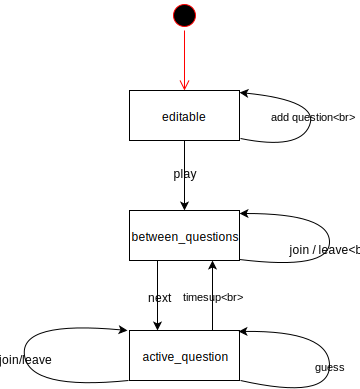
\includegraphics[width=0.8\textwidth]{images/Quizmaster}
\end{center}
	\caption{Simple drawing of the quizmaster state machine}
\end{figure}

\subsection{Data Structure}
Data with which we loop is a map with following entries:
\begin{itemize}
	\item \textbf{conductor} The Pid of the Conductor (Gamemaker)
	\item \textbf{questions} all questions which belong to a quiz
	\item \textbf{players} all joined players (we chose to either have active or inactive players (left the game) -> to get through the tests of OnlineTA -> just by guessing)
	\item \textbf{active\_question} The index of the active question (in the questions list)
	\item \textbf{answered} Saving the first guess for each player, to be sure only one guess can be made for each question
	\item \textbf{distribution} the distribution of the current active question which shows which index has be chosen how many times
\end{itemize}

\subsection{Editable state}
In the editable state the quiz can be modified, meaning new questions can be added or all existing questions can be retrieved.

\subsubsection{get\_questions}
Get all added questions.

\subsubsection{add\_question}
So the message add\_question adds a new question to the server state, with whom we loop further.
The question does have to in the format:
\begin{minted}{erlang}
[Description, [Answers]]
\end{minted}

In case the question doesn't fit the format we will get an error back that we tried to add a question in the wrong format


\subsection{Between\_questions state}
\subsection{Active\_question state}

needs to be improved

\section{Assessment}

\subsection{OnlineTA}
OnlineTA gave ok results back but only the last test wasn't able to fully run through and the end we ended up with guessing what exactly is wished what we implement to get through all test cases, so we gave up in th

\subsection{Scope of Test Cases}

\subsection{Correctness}

\subsection{Code Quality}


\appendix
\section{Code Listing}

\end{document}}